%% beamerthemeImperialPoster v1.0 2016/10/01
%% Beamer poster theme created for Imperial College by LianTze Lim (Overleaf)
%% LICENSE: LPPL 1.3
%%
%% This is the example poster demonstrating use
%% of the Imperial College Beamer Poster Theme
\documentclass[xcolor={table}]{beamer}
%% Possible paper sizes: a0, a0b, a1, a2, a3, a4 (although Imperial College posters are usually A0 or A1).
%% Possible orientations: portrait, landscape
%% Font sizes can be changed using the scale option.
\usepackage[size=a0,orientation=portrait,scale=1.55]{beamerposter}
\usepackage{amsmath} 						% Adds mathematical features for equations
\DeclareMathOperator{\Tr}{Tr}				% This is adding in a Trace definition for matrices
\usepackage{bbold}							% Adding in fancy letters for 1 operators etc.
\usepackage{mathtools}						% Adds in text for above/below arrows
\usepackage{physics} 						% Just for absolute values etc.
\usepackage{amssymb}						% For natural numbers symbol
\usepackage{dsfont}                         % for identity double stroke
\usepackage{wrapfig}
\usepackage{pstricks}
\usepackage[absolute,overlay]{textpos}
\renewcommand{\vec}{\vectorbold}            % if we want to redefine the vector 

\newcommand*{\field}[1]{\mathbb{#1}}%		% Defining the natural numbers
\newcommand*\dif{\mathop{}\!\mathrm{d}}		% Adding additional command for nice looking integration variables dx etc, use like " \dif variable " in integrals 
\newcommand*\bigO{\mathop{}\!\mathcal{O}}   % big O notation
\newcommand\ddfrac[2]{\frac{\displaystyle #1}{\displaystyle #2}}    % for creating bigger fractions that look nicer 

\definecolor{GraphRed}{HTML}{ec1c24}
\definecolor{GraphBlue}{HTML}{00a8f3}
\definecolor{GraphGreen}{HTML}{a1ecb6}
\definecolor{BackgroundBlue}{HTML}{d3e4f0}


\graphicspath{ {images/} }	

\usetheme{ImperialPoster}

%% Four available colour themes
\usecolortheme{ImperialWhite} % Default
% \usecolortheme{ImperialLightBlue}
% \usecolortheme{ImperialDarkBlue}
% \usecolortheme{ImperialBlack}

 
\title{\Huge Condensed Matter Theory}

% \setbeamertemplate{bibliography item}{\insertbiblabel}
% \addbibresource{supersolid.bib}

\begin{document}
\small
\begin{frame}[fragile=singleslide,t]\centering

\maketitle

\begin{tcolorbox}[colback=BackgroundBlue,colframe=ICDeepBlue,fontupper=\color{ICDeepBlue}]
\normalsize
    {\bf Condensed matter physics} is the study of an immense variety of solids and
    liquids found in nature or made by humans. Some of the things CMTH work on include metals, magnets, ceramics, graphene, superfluids, superconductors, polymers, complex liquids and planetary interiors. The Schr{\"o}dinger equation provides a ``grand unified theory'' on the atomic scale but on its own, an atom is a dull object. The behavior of assemblies of atoms, however, cannot be predicted from the individual properties of the atoms. Indeed, the study of emergent phenomena is a central theme of modern condensed matter physics. Those emergent behaviors are what give the world its astonishing diversity and richness.
\end{tcolorbox}

\begin{columns}[onlytextwidth,T]

%%%% First Column
\begin{column}{.47\textwidth}

\begin{block}{Metamaterials}
Imperial is the home of metamaterials, engineered materials with extraordinary abilities to guide and focus light in ways natural materials cannot. Sir John Pendry's revolutionary ideas are simple but change and expand our understanding of the world in profound ways.
Metamaterials exploit the idea that physically structuring on a scale less than the wavelength can dramatically alter a material’s property. Using man-made metamaterials, one can construct a perfect lens that, unlike a conventional lens, does not have limitations in the sharpness of the image or one can  create an invisibility cloak that guides light around an object, see Fig. 1. Metamaterials have transformed many areas of electromagnetism \& acoustics,  also commercially. Currently we are working on understanding time-dependent metamaterials where further phenomena emerge.
\end{block}
\vspace*{-1.5cm}
\begin{figure}
\centering
    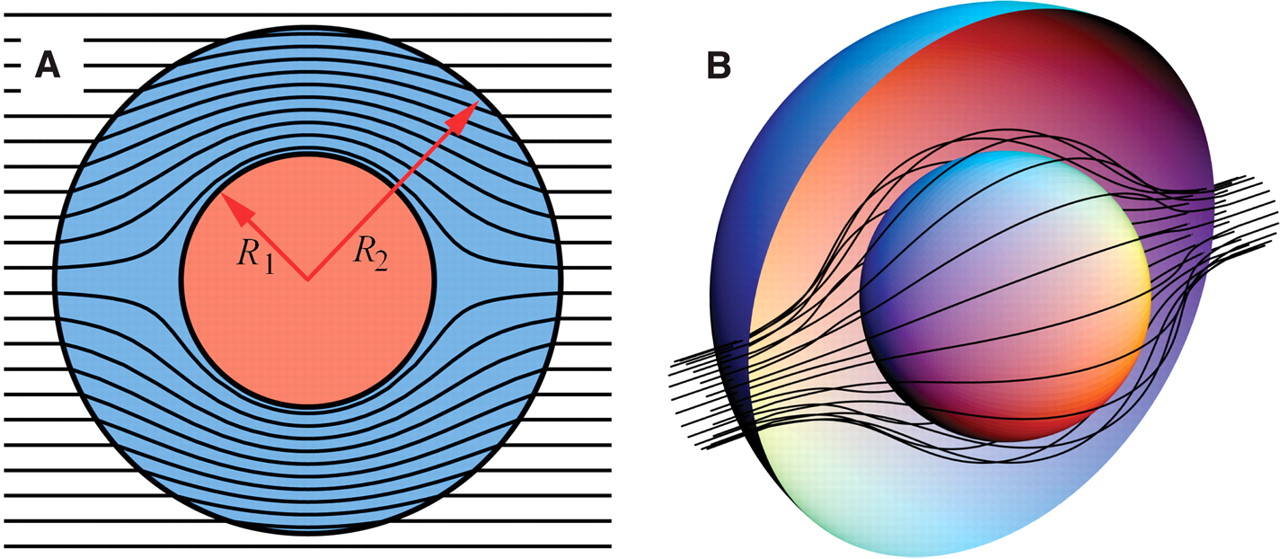
\includegraphics[width=0.9\columnwidth]{Cloak.jpeg}
    \caption{\footnotesize \textcolor{black}{Fig. 1. Pendry {\it \footnotesize et al.} [Science {\bf \footnotesize 312}, 5781 (2006)] proposed a way to guide light around an object using metamaterials with exotic optical properties. (A) Two-dimensional and (B) three dimensional view of microwave rays, where the cloaking material is present for $R_1 < R < R_2$. The invisibility cloak deflects microwave beams as they flow around an object hidden inside it, in the same way that water in a river flows around a pebble.}}
\end{figure}

\begin{block}{Complexity Science}

The richness and complexity in condensed matter physics reflects the fact that
new phenomena emerge on larger scales from the collective behaviour of simple
interacting objects on smaller scales, whether they are electrons in a metal or agents in a network. With colleagues at the Centre of Complexity Science, we have developed and applied transferable tools and techniques to real-world systems in many different contexts: geology (earthquake \& reservoir
engineering), atmospheric physics (rain), biology (evolution \& social insects), fire safety (smouldering), and medicine (brain \& heart). Currently we are working on econophysics, higher-order interactions in social networks and modelling atrial fibrillation.
\end{block}
\vspace*{-1.5cm}
\begin{figure}
    \centering
    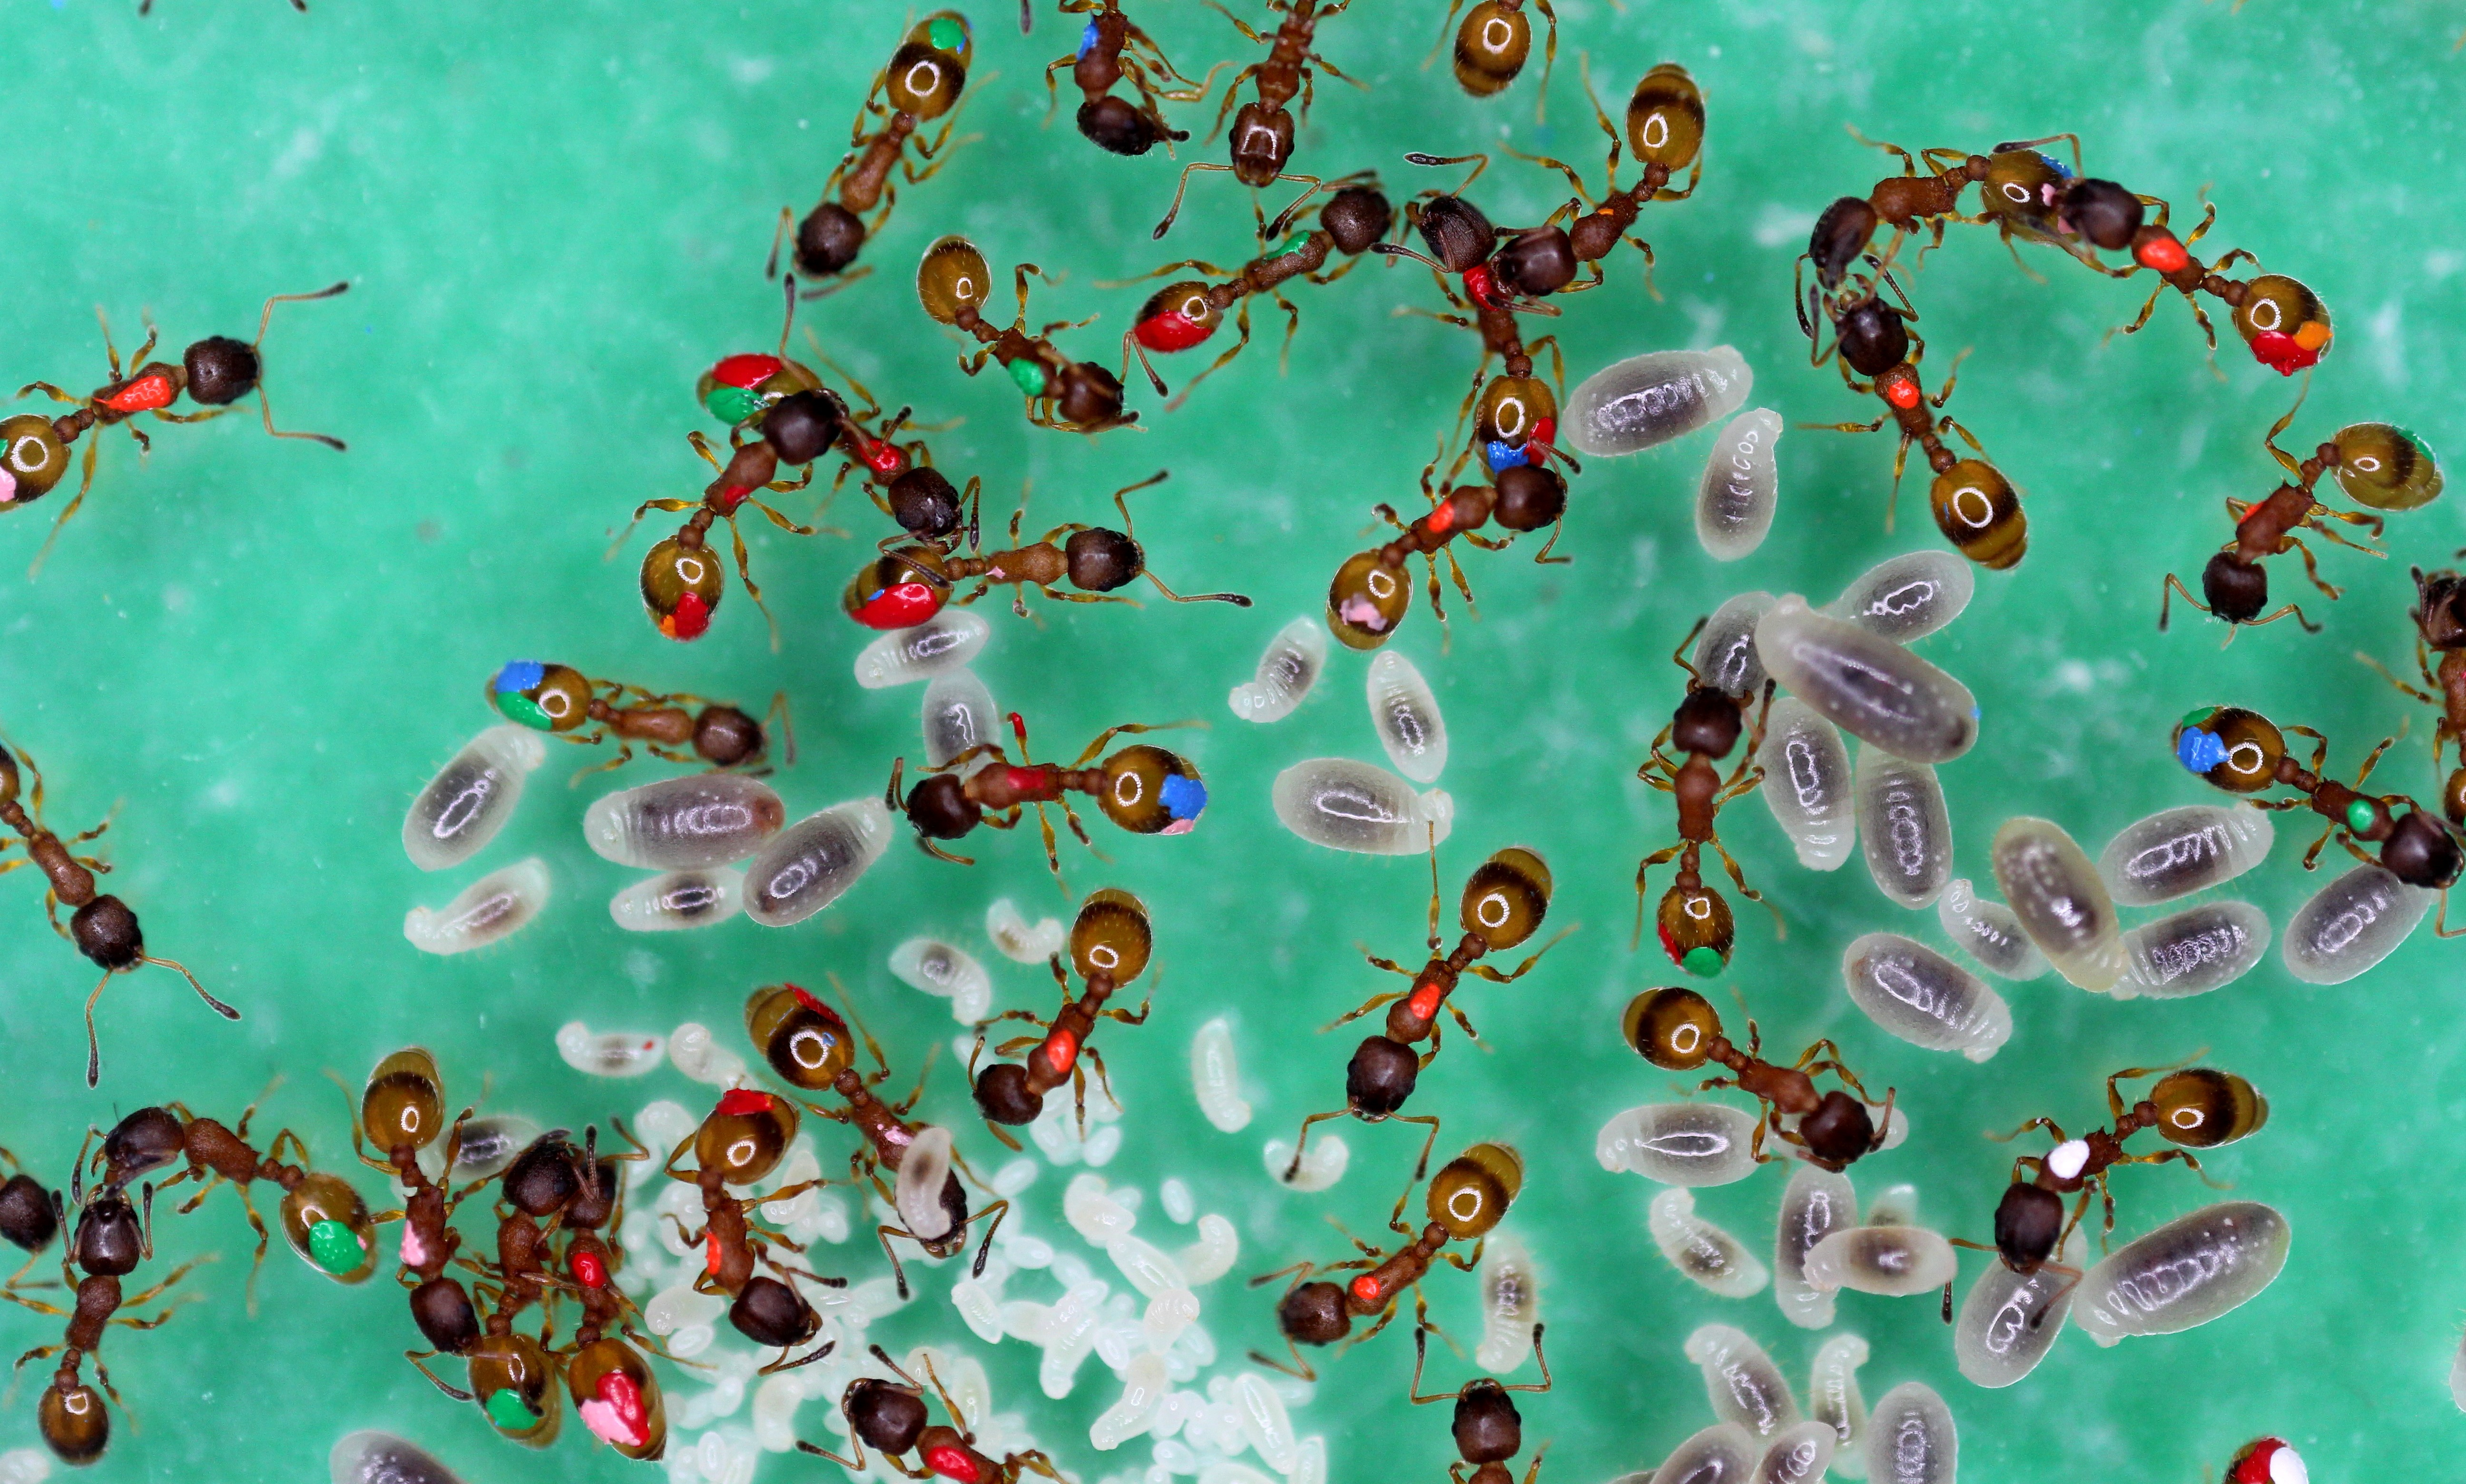
\includegraphics[width=0.9\columnwidth]{Temnothorax-albipennis-copyright-Nigel-R-Franks.jpg}
    \caption{\footnotesize \textcolor{black}{Fig. 2. The ant colony is a perfect example of a complex system in Nature. This self-organised and adaptive society's colony-level properties originate from interactions among the individual ants and the environment. Without ``top-down'' control, the self-organising ``bottom-up'' super-organism can accomplish incredible feats (e.g. that would be impossible for an individual ant. Photo of {\it \footnotesize  Temnothorax albipennis} ant colony courtesy of Nigel R Franks $\copyright$}}
\end{figure}

\end{column}

%%%% Second Column
\begin{column}{.47\textwidth}

\begin{block}{Correlated Quantum Systems}
Quantum mechanics is the reason why electrons, atoms, and molecules behave the way they do at the nanoscale. In turn, this affects the macroscopic properties of materials, such as electrical conduction in semiconductors, metals, and superconductors. The particle-wave duality of electrons and atoms becomes important at the nanoscale. Unlike other waves, like sound or light, which normally interact weakly with each other, electrons and atoms can interact quite strongly with each other. Our work encompasses a wide variety of different correlated quantum systems, like liquid helium films, ultracold atomic clouds, warm dense matter, and the emergence of new quantum phases of matter. We also use topology, which is a branch of geometry, to predict and characterise new forms of matter. Some of these new forms of matter even offer topologically protected qubits, which is the basic unit of information in a quantum computer.
\end{block}
\vspace*{-1.5cm}
\begin{figure}
\centering
    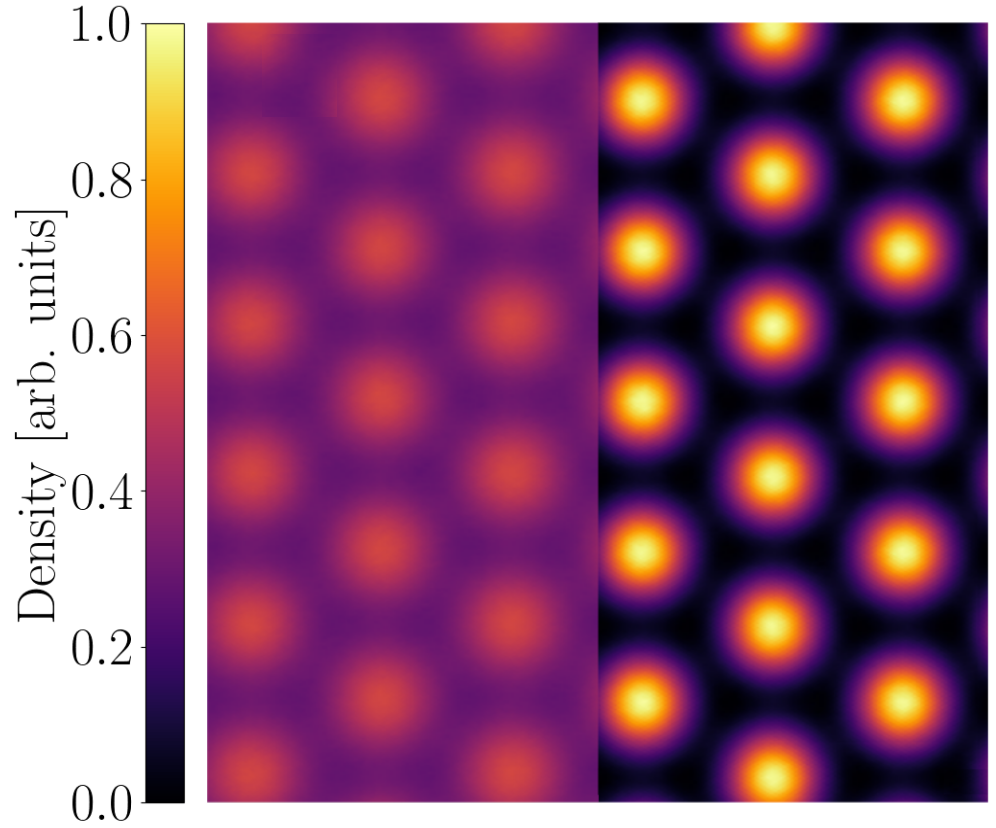
\includegraphics[width=0.52\columnwidth]{crystallisation.png}
    \caption{\footnotesize \textcolor{black}{Fig. 3. We are pioneering a new way to solve the Schr{\"o}dinger equation by representing the wavefunction as a deep neural network. The deep neural network (with parameters optimised internally via the variational principle) can span the quantum phase transition from a Fermi liquid at high density (left) to a Wigner crystal at low density (right).}}
\end{figure}

\begin{block}{Physics of Materials}
The development of civilisation would not have been possible without new materials. CMTH is at the forefront of research in this area, and our joint positions with the Department of Materials at Imperial mean that we are at the cutting edge of knowledge. We have also been pivotal for the Thomas Young Centre, which is dedicated to solving the scientific and technological challenges of today and the future. The goal is to solve the Schr{\"o}dinger equation or approximations thereof. We have developed computational codes that are used by hundreds of scientists around the world to solve the equations of quantum mechanics to predict the electronic behaviour of materials at the nanoscale, structural properties at the mesoscale, or material behaviour on the macroscale.
\end{block}
\vspace*{-1.5cm}
\begin{figure}
\centering
    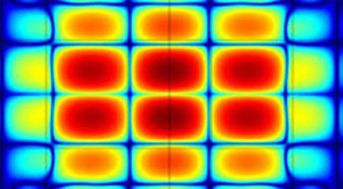
\includegraphics[width=0.9\columnwidth]{simulation_materials.jpg}
    \caption{\footnotesize \textcolor{black}{Fig. 4. This is only a figure holder. Please insert new relevant figure + associated caption here.}}
\end{figure}

\end{column}
\end{columns}

\begin{tcolorbox}[colback=BackgroundBlue,colframe=ICDeepBlue,fontupper=\color{ICDeepBlue}]
The Condensed Matter Theory team at Imperial is engaged in the intriguing adventure of investigating, understanding and even changing our fascinating natural world. For a showcase of particular projects, please see our posters in the hall of the Blackett Laboratory on Level 8 or visit www.imperial.ac.uk/condensed-matter-theory/
\end{tcolorbox}

% \put(10){
\includegraphics[height=2cm,
% width=2cm]{QR_code_for_mobile_English_Wikipedia.svg.png}}


\begin{textblock*}{10cm}(3cm,112cm) % {block width} (coords)
Centre for Complexity Science

\includegraphics[height=5cm, width=5cm]{QR_code_for_mobile_English_Wikipedia.svg.png}
\end{textblock*}
\end{frame}
\end{document}